\documentclass{article}
\usepackage{graphicx} % Required for inserting images
\usepackage[left=1.2in,right=1.2in,top=1in,bottom=1in]{geometry}
\usepackage{amsthm, amsfonts, amsmath, amssymb}
\usepackage{enumitem}
\usepackage[normalem]{ulem}
\usepackage{xcolor}
\usepackage{float}
\usepackage{hyperref}
\hypersetup{
    colorlinks=true,
    citecolor=blue,
    filecolor=black,
    linkcolor=blue,
    urlcolor=blue
}

\usepackage{marginnote} % 页边文字
\reversemarginpar
\newenvironment{note}[1]%
{%
  \def\notename{#1}% store argument in macro
  \marginnote{\fbox{\texttt{\notename}}}[0cm]%
  \label{\notename}
  \par\smallskip\noindent\ignorespaces
}
{\par\smallskip}
% define amsthm
\newtheorem{definition}{Definition}[section]
\newtheorem{proposition}{Proposition}[section]
\newtheorem*{lemma}{Lemma}
\newtheorem{theorem}{Theorem}[section]
\newtheorem*{remark}{Remark}

\setlength{\parindent}{0pt}

% define new command
\newcommand{\R}{\mathbb{R}}
\newcommand{\C}{\mathbb{C}}
\newcommand*{\dif}{\mathop{}\!\mathrm{d}}
\renewcommand{\labelitemi}{\scriptsize$\bullet$}

\title{Le Gall: Measure Theory, Probability, \\and Stochastic Processes\\ Companion Notes}
\author{Taken by: Mark Zhu}
\date{August 2025}

\begin{document}

\maketitle
\tableofcontents
\newpage

\part{Measure Theory}
\setcounter{section}{0}
\section{Measurable Spaces}
\begin{note}{Def 1.2}
    $\mathcal{C}$ is a collection of subsets of $E$.
\end{note}

\begin{note}{p.~4}
    ``Clearly, closed subsets of $E$ are Borel sets.'' 
    
    Let $U\subset E$, and $U$ is open $\implies U\in\mathcal{B}(E)$. Since $\mathcal{B}(E)$ is a $\sigma$-field, $E\setminus U\in \mathcal{B}(E)$, which is closed.
\end{note}

\begin{note}{Lem 1.5}
    To prove $\mathcal{B}(E)\otimes \mathcal{B}(F)\subset \mathcal{B}(E\times F)$, consider the following class
    \[\mathcal{C}_B=\{A\in \mathcal{B}(E):A\times B\in \mathcal{B}(E\times F)\}\]
    Fix $B\subset F$ be open. $\mathcal{B}(E\times F)=\sigma(\mathcal{O})$ where $\mathcal{O}=\{\text{all open subsets of }E\times F\}$, and $E\times F=\{(e,f): e\in E,f\in F\}$. If $A\subset E$ is also open, then $A\times B\in \mathcal{B}(E\times F),A\in \mathcal{C}_B,\mathcal{B}(E)\subset \mathcal{C}_B$. Clearly $\mathcal{C}_B\subset \mathcal{B}(E)$, so $\mathcal{C}_B=\mathcal{B}(E)$.
\end{note}

\begin{note}{p.~7}
    In the proof of property (4), discuss why
    \[
    \mu\left(
    B_1\setminus \bigcap_{n\in \mathbb{N}}B_n
    \right)=\mu\left(
    \bigcup_{n\in \mathbb{N}}A_n
    \right)
    \]
    Derive $B_1\setminus \bigcap_{n\in \mathbb{N}}B_n=B_1\cap(\bigcap_{n\in \mathbb{N}}B_n)^c=B_1\cap(\bigcup_{n\in \mathbb{N}}B_n^c)=\bigcup_{n\in \mathbb{N}}(B_1\cap B_n^c)=\bigcup_{n\in \mathbb{N}}A_n$.
\end{note}

\begin{note}{p.~9}
    Discuss the equivalence of limsup and liminf for sequences of numbers $\{a_n\}$ and of sets $\{A_n\}$. Recall
    \[
    \limsup_{n\to\infty}\{a_n\}=\lim_{n\to\infty}\sup_{k\ge n}\{a_k\},\quad \limsup_{n\to\infty}A_n=\bigcap_{n=1}^{\infty}\bigcup_{k=n}^{\infty}A_k
    \]
    Define an indicator function
    \[
    a_n(x)=\begin{cases}
        1 & x\in A_n\\
        0 & x\notin A_n
    \end{cases}
    \]
    $\sup_{k\ge n}\{a_k(x)\}=1$ if $\exists k\ge n$ such that $x\in A_k$. $\sup_{k\ge n}\{a_k(x)\}=0$ otherwise. Take limits, then $\lim_{n\to\infty}\sup_{k\ge n}\{a_k\}=1$ if $\forall n\ge 1,\exists k\ge n$ such that $x\in A_k$. 
    
    Note that $\forall n\ge 1\iff \bigcap_{n\ge 1}$; $\exists k\ge n\iff \bigcup_{k\ge n}$, so
    \[
    \limsup_{n\to\infty}\{a_n(x)\}=\begin{cases}
        1 & x\in \bigcap_{n=1}^{\infty}\bigcup_{k=n}^{\infty}A_k\\
        0 & \text{otherwise}
    \end{cases}
    \]
    For liminf, it's more natural to consider the inverse statement. $\inf_{k\ge n} \{a_k(x)\}=0$ if $\exists k\ge n$ such that $x\notin A_k$, so $a_k(x)=0$. $\lim_{n\to\infty}\inf_{k\ge n}\{a_k\}=0$ if $\forall n\ge 1,\exists k\ge n$ such that $x\notin A_k$. That means if $\exists n\ge 1,\forall k\ge n, x\in A_k$, then $\lim_{n\to\infty}\inf_{k\ge n}\{a_k\}=1$. Thus
    \[
    \liminf_{n\to\infty}\{a_n(x)\}=\begin{cases}
        1 & x\in \bigcup_{n=1}^{\infty}\bigcap_{k=n}^{\infty}A_k\\
        0 & \text{otherwise}
    \end{cases}
    \]
    Conclusion: the gap between real numbers and sets is closed by \emph{indicator functions}.
\end{note}

\begin{note}{Lem 1.7}
    Because $\bigcap_{k=n}^{\infty}A_k\subset A_k, $ for all $k\ge n$,
    \[
    \mu\left(\bigcap_{k=n}^{\infty}A_k\right)\le \mu(A_k)
    \]
    So $\mu\left(\bigcap_{k=n}^{\infty}A_k\right)\le \inf_{k\ge n}\mu(A_k)$. Since $\bigcap_{k=n}^{\infty}A_k$ is increasing with respect to $n$, use property (3) in p. 6, and get the desired result.
\end{note}

\begin{note}{Prop 1.10}
    To let $f$ measurable, two conditions should suffice
    \begin{enumerate}
        \item $\exists $ generator $\mathcal{C}\subset \mathcal{B}$, such that $\sigma(\mathcal{C})=\mathcal{B}$
        \item $f$ is measurable on $\mathcal{C}$
    \end{enumerate}
    By Def 1.8 and the second condition, $\forall B\in \mathcal{C},f^{-1}(B)\in \mathcal{A}$. So $B\in \mathcal{G},\mathcal{C}\subset\mathcal{G}$. Now show that $\mathcal{G}$ is a $\sigma$-field.
    \begin{itemize}
        \item $F\in\mathcal{B},f^{-1}(F)=E\in \mathcal{A}\implies F\in \mathcal{G}$
        \item Let $B\in \mathcal{G}$, so $f^{-1}(B)\in \mathcal{A}$. Since $\mathcal{A}$ is a $\sigma$-field, $\mathcal{A}\ni E\setminus f^{-1}(B)=f^{-1}(F\setminus B)$, so $B^c=F\setminus B\in \mathcal{G}$
        \item If $B_n\in \mathcal{G}$, then $f^{-1}(B_n)\in \mathcal{A},f^{-1}(\bigcup_{n\ge 1} B_n)=\bigcup_{n\ge 1} f^{-1}(B_n)\in \mathcal{A}$. So $\bigcup_{n\ge 1} B_n\in \mathcal{G}$
    \end{itemize}
    So $\mathcal{G}$ is a $\sigma$-field. Since $\mathcal{C}\subset\mathcal{G}$, $\mathcal{B}=\sigma(\mathcal{C})\subset\mathcal{G}$. By construction of $\mathcal{G}$, $\mathcal{G}\subset \mathcal{B}$. Thus $\mathcal{G}=\mathcal{B}\implies \forall B\in \mathcal{B},f^{-1}(B)\in \mathcal{A}$, so $f$ is measurable.
\end{note}

\begin{note}{Lem 1.15}
\begin{enumerate}
    \item ``The set $A$ of all $x\in E$ such that $f_n(x)$ converges in $\mathbb{R}$ as $n\to\infty$ is measurable'' where `converges' means $\limsup_n f_n=\liminf_nf_n$. 

    \item $A=G^{-1}(\Delta)$ is followed by $\Delta$ is a measurable set, $G$ is a measurable function, so $G^{-1}(\Delta)\in\mathcal{A}$ under measurable space $(E,\mathcal{A})$.

    \item Then move on to the second statement that $h:E\to\mathbb{R}$ is measurable. If $\forall F\subset \mathbb{R}, h^{-1}(F)\in \mathcal{A}$, i.e. $h^{-1}(F)$ is a measurable set, then $h$ is a measurable function. 
    
    (Case 1) If $0\notin F$, then $h$ collapses into $h(x)=\lim_n f_n(x),\forall x\in A$. Then $h^{-1}(F)$ is given by
    \[
    h^{-1}(F)=A\cap \{x\in E:\limsup f_n(x)\in F\}
    \]
    and both sets on the right are measurable.
    
    (Case 2) If $0\in F$, then $0\notin F^c$.
    \[
    x \in (h^{-1}(F))^c \iff h(x) \notin F \iff h(x) \in F^c \iff x \in h^{-1}(F^c)
    \]
    which means $(h^{-1}(F))^c=h^{-1}(F^c)$. From Case 1 we know $h^{-1}(F^c)$ is a measurable set, so does $(h^{-1}(F))^c$. Because the collection of measurable sets is a $\sigma$-field (by Def 1.1), $h^{-1}(F)$ is also measurable.
\end{enumerate}
\end{note}

\begin{note}{p.~13}
    ``Any $\sigma$-field is also a monotone class. Conversely, a monotone class $\mathcal{M}$ is a $\sigma$-field if and only if it is closed under finite intersections.''

    Question: How `closure under finite intersections' helps $\mathcal{M}$ becoming a $\sigma$-field?

    For property (ii), set $B=E$, then $A^c=E\setminus A\in \mathcal{M}$. For property (iii), given $\mathcal{M}$ is closed under finite intersections, let $A,B\in \mathcal{M}, A^c\cap B^c\in\mathcal{M}\implies A\cup B=(A^c\cap B^c)^c$. So it's also closed under finite union. Define
    \[
    B_n=\bigcup_{k=1}^n A_k
    \]
    clearly $B_n\subset B_{n+1}$. Apply (iii), 
    \[
    \mathcal{M}\ni\bigcup_{n\in\mathbb{N}}B_n=\bigcup_{n\in\mathbb{N}}\bigcup_{k=1}^n A_k=\bigcup_{k\in\mathbb{N}} A_k
    \]
    without the restriction of $A_n\subset A_{n+1}$.
\end{note}

\begin{note}{Thm 1.18}
    Explanation about the proof
    \begin{enumerate}
        \item When verifying $\mathcal{M}_A$ is a monotone class, in the complement property
        \[
        \mathcal{M}(\mathcal{C})\ni(A\cap B')\setminus (A\cap B)=A\cap(B'\setminus B)
        \]
        is based on the construction of $\mathcal{M}_A$ and nothing else.
        \item Before the last step, we reached the result
        \[
        \forall A\in \mathcal{C},\forall B\in \mathcal{M}(\mathcal{C}),A\cap B\in \mathcal{M}(\mathcal{C})
        \]
        But to show $\mathcal{M}(\mathcal{C})$ is closed under finite intersections, we need 
        \[
        \forall A,B\in \mathcal{M}(\mathcal{C}),A\cap B\in \mathcal{M}(\mathcal{C})
        \]
        Previously, we fixed $A\in \mathcal{C}$ to reach the property $\mathcal{C}\subset \mathcal{M}_A$ and everything follows. So we cannot simply replace $A\in \mathcal{C}$ by $A\in \mathcal{M}(\mathcal{C})$. Here's what we do:

        Fix $B\in \mathcal{C}$. Now $A$ can be an arbitrary set in $\mathcal{M}(\mathcal{C})$. Use the conclusion above, $A\cap B\in \mathcal{M}(\mathcal{C})$, so $B\in \mathcal{M}_A$. That is, $\forall B\in \mathcal{C}, B\in \mathcal{M}_A$, thus $\mathcal{C}\subset \mathcal{M}_A,\forall A\in\mathcal{M}(\mathcal{C})$. Since $\mathcal{M}_A$ is a monotone class, $\mathcal{M}(\mathcal{C})\subset \mathcal{M}_A$, $\mathcal{M}(\mathcal{C})$ is closed under finite intersection.
    \end{enumerate}
\end{note}

\begin{note}{Cor 1.19}
    In (1), $\mu(E) = v(E)$ ensures that $\mathcal{G}$ satisfies its first property for being a monotone class. In (2), $\mu_n,v_n$ are respective restrictions of $\mu,v$ to $E_n$, i.e. 
    \[\mu_n(A)=\mu(A\cap E_n),\quad \forall A\in \mathcal{A}\]
    $\mu(E_n)=v(E_n)$ allows us to apply (1) to $\mu_n,v_n$, $\implies \mu_n=v_n$. Then
    \[
    \mu(A)=\mu(A\cap E)=\mu\left(A\cap \bigcup_{n\in\mathbb{N}}E_n\right)=\mu\left(\bigcup_{n\in\mathbb{N}}(A\cap E_n)\right)=\lim_{n\to\infty}\uparrow \mu(A\cap E_n)
    \]
    by property (3) in p. 6, where $A\cap E_n$ is increasing.
\end{note}
\setcounter{section}{1}
\section{Integration of Measurable Functions}

\begin{note}{Prop 2.3}
    Rigorously prove property (2). Let $h\in\mathcal{E}_+$ such that $h\le f$. Then if $h(x)>0, f(x)\ge h(x)>0$, so
    \[
    \{x\in E: h(x)>0\}\subset \{x\in E: f(x)>0\}
    \]
    Given $\mu(\{x\in E: f(x)>0\})=0$, so $\mu(\{x\in E: h(x)>0\})=0$. The integral of $h$ would be
    \[
    \int h\mathrm{d}\mu=\sum_{i=1}^n \alpha_i\mu(A_i)=0
    \]
    since either $\alpha_i=0$ or $\alpha_i>0$ but $\mu(A_i)=0$. Because $h\le f$ always holds,
    \[
    \int f\mathrm{d}\mu=\sup_{h\le f} \int h\mathrm{d}\mu=0
    \]
\end{note}

\begin{note}{Thm 2.4}
    \begin{enumerate}
        \item Why is $f$ measurable? 
        
        $f_n\to f\implies f=\limsup f_n=\liminf f_n$, then by Prop 1.14.
        \item Why $\int f \mathrm{d}\mu\ge \lim_n \int f_n \mathrm{d}\mu$? 
        
        Since $f_n$ is increasing, $f_n\le \lim_n f_n=f$. Take integrals, $\int f \mathrm{d}\mu\ge \int f_n \mathrm{d}\mu$, then take limit $n\to\infty$ on the RHS.
        \item Why $f_n\to f,a<1$ leads to $E_n\uparrow E$?

        We want to prove (1) $E_n\subset E_{n+1},\forall n$, (2) $\bigcup_{n=1}^{\infty}E_n=E$.

        (1) Take $x\in E_n, ah(x)\le f_n(x)\le f_{n+1}(x)$, so $x\in E_{n+1}$.

        (2) Let $x\in E,h(x)\le f(x),0\le a<1$. 
        \begin{enumerate}
            \item $h(x)=0$. Then $ah(x)=0\le f(x)$, so $x\in E_n,\forall n$.
            \item $h(x)>0$. Then $ah(x)<h(x)\le f(x)$. Since $f_n(x)\uparrow f(x), \exists N\in \mathbb{N}$, such that for $n\ge N,ah(x)<f_n(x)$. Thus $\forall n\ge N, x\in E_n$.
        \end{enumerate}
        We conclude that, $\forall x\in E,\exists N\in\mathbb{N}$, such that $\forall n\ge N,x\in E_n$, so
        \[\bigcup_{n\in\mathbb{N}}E_n=E\]
        Combined with $E_n\subset E_{n+1}, E_n\uparrow E$.
        \item Given $f_n\ge a\mathbf{1}_{E_n}h,$ then
        \[
        \int a\mathbf{1}_{E_n}h\mathrm{d}\mu=\int a\mathbf{1}_{E_n}\left(\sum_{i=1}^k \alpha_i \mathbf{1}_{A_i}\right)\mathrm{d}\mu=\int \left(a\sum_{i=1}^k \alpha_i \mathbf{1}_{E_n\cap A_i}\right)\mathrm{d}\mu=a\sum_{i=1}^k \alpha_i\mu(E_n\cap A_i)
        \]
        \item In the last step 
        \[
        \int h\mathrm{d}\mu\le \lim_{n\to\infty}\uparrow \int f_n \mathrm{d}\mu
        \]
        take $\sup_{h\in \mathcal{E}_+,h\le f}$ on both sides.
        \item Conclusion: 
        
        The most insightful part of this proof is to construct a simple function $h=\sum_{i=1}^k \alpha_i \mathbf{1}_{A_i}$ and restrict $h\le f$, then use Def 2.2.
    \end{enumerate}
\end{note}

\begin{note}{Prop 2.5}
    The author used constructive proof for (1). Recall uniform convergence: $\forall \varepsilon>0,\exists N\in\mathbb{N}$ such that $\forall n\ge N, x\in E, |f_n(x)-f(x)|<\varepsilon$. In uniform convergence, $N$ cannot depend on $x$. The constructed $f_n$ satisfies $0\le f-f_n\le 2^{-n}$ where $2^{-n}$ does not depend on $x$. 

    Example: $f(x)=2\sin(x)+2,n=3$, see Fig \ref{fig:prop2.5}.
    \begin{figure}[htbp]
        \centering
        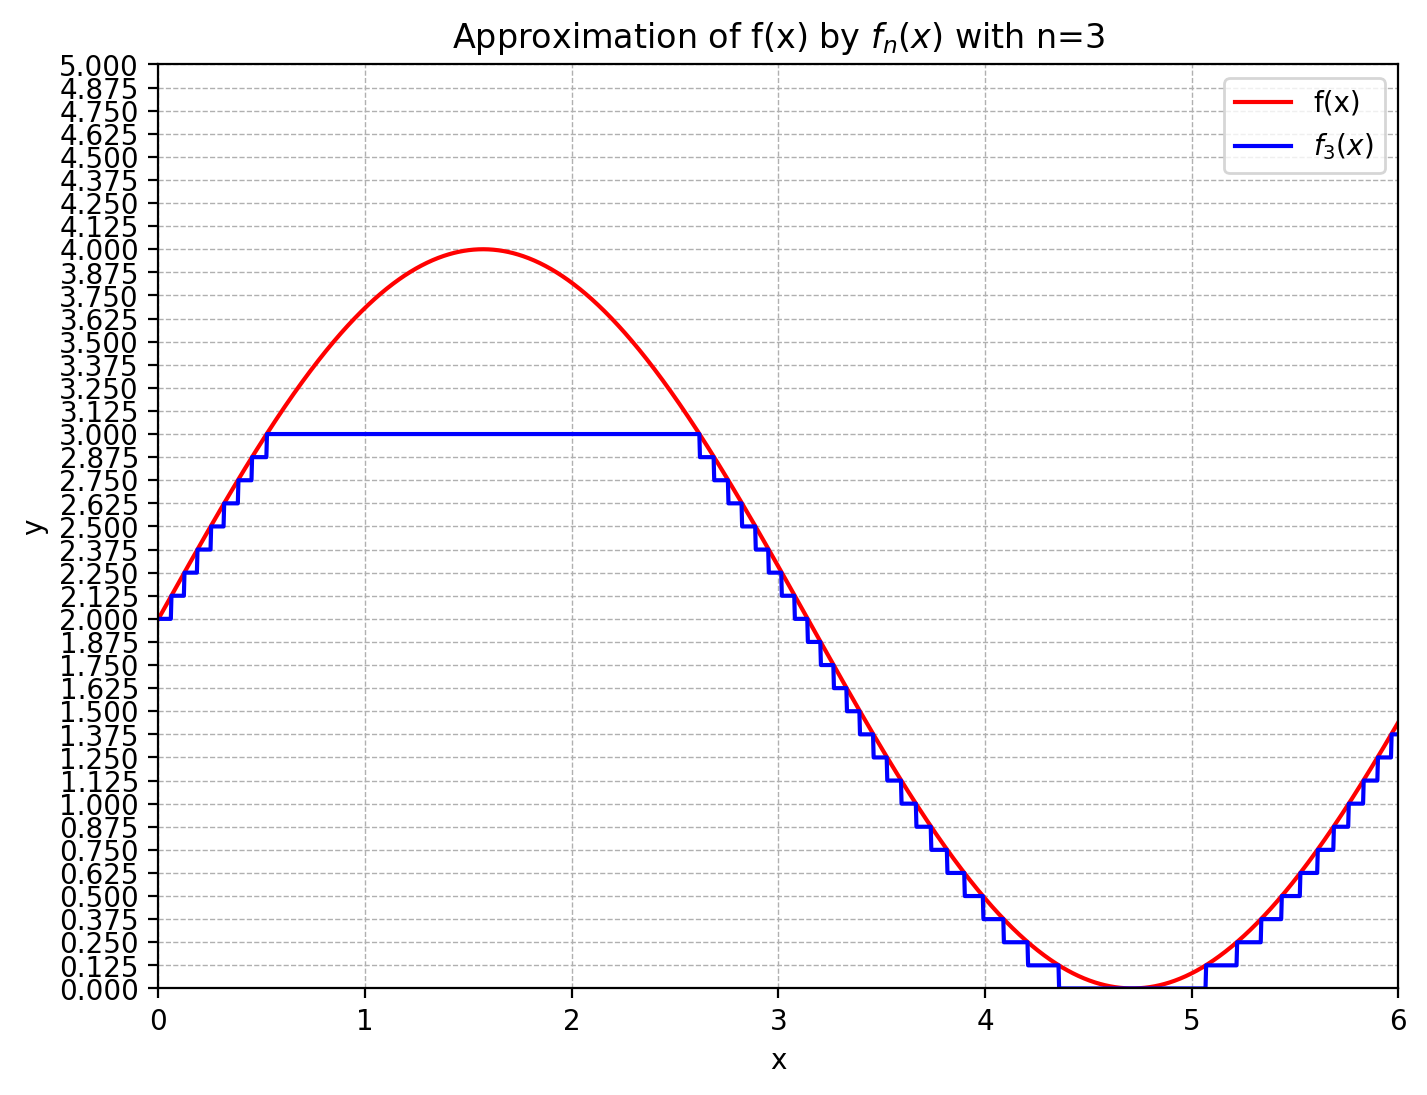
\includegraphics[width=0.6\linewidth]{fig/prop2-5.png}
        \caption{Example for Prop 2.5(1)}
        \label{fig:prop2.5}
    \end{figure}
\end{note}

\begin{note}{p.~23}
    Counting measure is simply summing up, analogously, \texttt{np.sum(x)} in numpy. 
    \begin{enumerate}
        \item $f_n(k)=f(n)\mathbf{1}_{\{n\}}(k)$, which means only when $k=n$ does $\mathbf{1}_{\{n\}}(k)=1$, thus $\sum_n f_n(k)=\sum_n f(n)\mathbf{1}_{\{n\}}(k)=f(k)$ (fix $k$ and treat $n$ as the variable). So $\sum_n f_n=f$. By Prop 2.5(3),
        \[
        \int f\mathrm{d}\mu=\int \left(\sum_{n\in\mathbb{N}}f_n\right)\mathrm{d}\mu=\sum_{n\in\mathbb{N}}\int f_n\mathrm{d}\mu
        \]
        Since $f_n$ is a simple function,
        $$
        \int f_n\mathrm{d}\mu=\int f(n)\mathbf{1}_{\{n\}}(k)\mathrm{d}\mu(k)=\sum_{k\in\mathbb{N}}f(n)\mathbf{1}_{\{n\}}(k)=f(n)
        $$
        We conclude that
        \[
        \int f\mathrm{d}\mu=\sum_{n\in\mathbb{N}}f(n).
        \]
        \item $f_n(k)=a_{n,k}$, remember that $k$ is the variable.
        \[
        \int\left(\sum_{n\in\mathbb{N}}f_n\right)\mathrm{d}\mu=
        \int\left(\sum_{n\in\mathbb{N}}a_{n,k}\right)\mathrm{d}\mu=
        \sum_{k\in\mathbb{N}}\left(\sum_{n\in\mathbb{N}}a_{n,k}\right)
        \]
        \[
        \sum_{n\in\mathbb{N}}\int f_n\mathrm{d}\mu=
        \sum_{n\in\mathbb{N}}\int a_{n,k}\mathrm{d}\mu=
        \sum_{n\in\mathbb{N}}\left(\sum_{k\in\mathbb{N}}a_{n,k}\right)
        \]
        Then use Prop 2.5(3).
    \end{enumerate}
\end{note}

\begin{note}{Cor 2.6}
    Detailed proof for equation (2.1). 
    \begin{itemize}
        \item[(Step 1)] For indicator function $f=\mathbf{1}_A$
        \[
        \int \mathbf{1}_A\mathrm{d}v=v(A)=\int \mathbf{1}_A g\mathrm{d}\mu
        \]
        by definition of integral (see Def 2.1) and $v(A)$.
        \item[(Step 2)] Extend to simple function using Prop 2.5(2),$f_n=\sum_{i=1}^n \alpha_i \mathbf{1}_{A_i}$,
        \[
        \int f_n\mathrm{d}v=\int \left(\sum_{i=1}^n \alpha_i \mathbf{1}_{A_i}\right)\mathrm{d}v=\sum_{i=1}^n\alpha_i\int \mathbf{1}_A\mathrm{d}v
        \]
        By Step 1,
        \[
        =\sum_{i=1}^n\alpha_i\int \mathbf{1}_A g\mathrm{d}\mu=\int f_n g\mathrm{d}\mu
        \]
        \item[(Step 3)] Extend to all nonnegative measurable function using Prop 2.5(1). $\exists \{f_n\}_n$ such that $f_n\uparrow f$. By Thm 2.4,
        \[
        \int f\mathrm{d}v=\lim_{n\to\infty}\uparrow \int f_n\mathrm{d}v=\lim_{n\to\infty}\uparrow \int f_n g\mathrm{d}\mu=\int f g\mathrm{d}\mu
        \]
    \end{itemize}
\end{note}

\begin{note}{Prop 2.7}
    (2) Logic: write $\infty$ as $\forall n\ge 1, \exists f(x)>n$. Call $\{f(x)>n\}$ an event, denoted by $A_n$. $\forall n\ge 1$ in set theory language is $\bigcap_{n\ge 1}$.

    Question: Does the reverse hold? Answer: No! Counterexample: $f(x)=1/x,x\in(0,1]$, and let $\mu$ be Lebesgue measure. $f<\infty$ a.e., but $\int_0^1 \frac{1}{x}\mathrm{d}x=\infty$.

    (3) To show the set such that $f(x)$ lies in $(0,+\infty)$ is measure zero, find a sequence of sets such that
    \[
    (0,+\infty)=\bigcup_{n=1}^{\infty}[1/n,+\infty)
    \]
\end{note}

\begin{note}{Prop 2.9}
    The proof appears extremely similar to Cor 2.6.
    \begin{enumerate}
        \item[(Step 1)] Let $h=\mathbf{1}_B$, then $h=1$ only when $\varphi(x)\in B, x\in \varphi^{-1}(B)$.
        \[
        \int_E \mathbf{1}_B (\varphi(x))\mu(\dif x)=\int_E \mathbf{1}_{\varphi^{-1}(B)} (x)\mu(\dif x)=\mu(\varphi^{-1}(B))=v(B)=\int_F \mathbf{1}_B(y)v(\dif y)
        \]
        \item[(Step 2)] If $h_n$ is a simple function, $h_n=\sum_{i=1}^n\alpha_i \mathbf{1}_{A_i}$.
        \[
        \int_E h_n(\varphi(x))\mu(\dif x)
        =\sum_{i=1}^n \alpha_i\int_E \mathbf{1}_{A_i}(\varphi(x))\mu(\dif x)
        =\sum_{i=1}^n\alpha_i v(A_i)
        =\int_F h_n(y)v(\dif y)
        \]
        \item[(Step 3)] For all nonnegative measurable function $h$, contruct $h_n\uparrow h$ using the method in Prop 2.5(1). By Thm 2.4 (MCT),
        \[
        \int_E h(\varphi(x))\mu(\dif x)
        =\lim_{n\to\infty}\uparrow \int_E h_n(\varphi(x))\mu(\dif x)
        =\lim_{n\to\infty}\uparrow \int_F h_n(y)v(\dif y)
        =\int_F h(y)v(\dif y)
        \]
    \end{enumerate}
\end{note}

\begin{note}{p.~34}
    ``Notice that (iii)'$\Rightarrow$(iii) thanks to the mean value theorem.''

    $\exists\xi\in(u_0,u)$ or $\in (u,u_0)$, such that
    \[
    |f(u,x)-f(u_0,x)|\le \bigg|\frac{\partial f}{\partial u}(\xi,x)\bigg|\cdot |u-u_0|\le g(x)\cdot |u-u_0|
    \]
\end{note}
\setcounter{section}{2}
\section{Construction of Measures}

\begin{note}{Def 3.1}
    Can $\sigma$-subadditive $\Rightarrow \sigma$-additive? No. Counterexample: define
    \[
    \mu(A)=\begin{cases}
        1 & A\neq \varnothing\\
        0 & A=\varnothing
    \end{cases}
    \]
    Then $\forall \{A_k\}_k$,
    \[
    \mu\left(
    \bigcup_{k\ge 1}A_k
    \right)=\mathbf{1}_{\{\exists k: A_k\neq\varnothing\}}\le \sum_{k\ge 1}\mathbf{1}_{\{A_k\neq\varnothing\}}=\sum_{k\ge 1}\mu(A_k)
    \]
    so $\sigma$-subadditive holds. Take $A_k=\{x_k\}$, all disjoint, but
    \[
    \mu\left(
    \bigcup_{k\ge 1}A_k
    \right)=\mu(\{x_1,\cdots,x_n\})=1\neq \infty\impliedby\sum_{k\ge 1}\mu(A_k)=\sum_{k\ge 1}1
    \]
\end{note}

\begin{note}{Thm 3.3}
    (i) How does the author come up with equation (3.1) to prove (i)? We want to show $\bigcup_{k\in\mathbb{N}}B_k\in\mathcal{M}$, then show
    \[
    \mu^*(A)\ge \underbrace{\mu^*\left(
    A\cap \bigcup_{k\in\mathbb{N}}B_k
    \right)}_{(1)}+\underbrace{\mu^*\left(
    A\cap \left(\bigcup_{k\in\mathbb{N}}B_k\right)^c
    \right)}_{(2)}
    \]
    Apply De Morgan's Law on (2). For (1), rewrite it as 
    \[
    \mu^*\left(
    A\cap \bigcup_{k\in\mathbb{N}}B_k
    \right)=\mu^*\left(
     \bigcup_{k\in\mathbb{N}} (A\cap B_k)
    \right)
    \]
    and by $\sigma$-subadditive of $\mu^*$, 
    \[
    \le \sum_{k\in\mathbb{N}}\mu^*(A\cap B_k)
    \]
    So the minimal requirement is
    \[
    \mu^*(A)=\sum_{k\in\mathbb{N}}\mu^*(A\cap B_k)+\mu^*\left(
    A\cap \bigcap_{k\in\mathbb{N}}B_k^c\right)
    \]
    Plug in $k=1$ and check, $\mu^*(A)=\mu^*(A\cap B_1)+\mu^*(A\cap B_1^c)$, meaning the equation is very likely to hold, then we can safely explore the proof.

    (ii) $\mathcal{M}(\mu^*)\subset \mathcal{P}(E)$, restriction of $\mu^*$ to $\mathcal{M}$ simply changes the domain of $\mu^*$ from $\mathcal{P}(E)$ to $\mathcal{M}$, maintaining the value unchanged. So for $\mu:=\mu^*|_{\mathcal{M}}$,
    \[
    \mu: \mathcal{M}\to [0,+\infty],\quad \mu(B)=\mu^*(B), \forall B\in \mathcal{M}
    \]
\end{note}

\begin{note}{p.~44}
    ``The infimum is over all countable covers of $A$ by open intervals $(a_i,b_i),i\in\mathbb{N}$ (it is trivial that such covers exist).'' This is not trivial, it's \emph{Heine-Borel Theorem}.
\end{note}

\begin{note}{p.~46}
\begin{enumerate}
    \item Summing up the two inequalities, the RHS gives,
    \[
    \begin{aligned}
        \relax[(b_i\land \alpha)-(a_i\land \alpha)]+[(b_i\lor \alpha)-(a_i\lor \alpha)]&=[(b_i\land \alpha)+(b_i\lor \alpha)]-[(a_i\land \alpha)+(a_i\lor \alpha)]\\
        &=(b_i+\alpha)-(a_i+\alpha)=b_i-a_i
    \end{aligned}
    \]
    \item By Lem 3 in the lecture note \href{https://ocw.mit.edu/courses/18-s190-introduction-to-metric-spaces-january-iap-2023/mit18_s190iap23_lec4.pdf}{MIT18.S190 Lec4}, that a metric space $X$ being sequentially compact implies that $X$ is \emph{totally bounded} ($\forall \varepsilon>0,\exists x_1,\cdots,x_k\in X$ with finite $k$ such that $\{B_{\varepsilon}(x_i)\}_k$ is an open cover of $X$). It follows $\exists N, [a,b]\subset \bigcup_{i=1}^N (a_i,b_i)$.
\end{enumerate}
\end{note}

\begin{note}{Prop 3.6}
    $\mathcal{N}$ shows the situation when a set $A\notin\mathcal{A}$ but it's small enough to be negligible. Another name for $\bar{A}$ is \emph{completion}, and this proposition says there exists a unique extended measure that (1) gives the same value for all sets in $\mathcal{A}$, and (2) assigns zero measure to all sets in $\mathcal{N}$.
    \begin{enumerate}
        \item Verify that $\mathcal{B}$ is a $\sigma$-field
        \begin{enumerate}
            \item Let $B=B'=E\in\mathcal{A}, \mu(E\setminus E)=0\implies E\in\mathcal{B}$.
            \item If $A\in\mathcal{B}$, then $\exists B,B'\in\mathcal{A}, B\subset A\subset B',\mu(B'\setminus B)=0$. $B^c\supset A^c\supset B'^c,\mu(B^c\setminus B'^c)=\mu(B^c\cap B')=\mu(B'\setminus B)=0$. So $A^c\in\mathcal{B}$.
            \item If $A_n\in\mathcal{B},\forall n\ge 1$, then $\exists B_n,B_n'\in\mathcal{A}, B_n\subset A_n\subset B_n',\mu(B_n'\setminus B_n)=0$. Let $B:=\bigcup_{n\ge 1}B_n\subset \bigcup_{n\ge 1}A_n\subset \bigcup_{n\ge 1}B_n'=:B'$,
            \[
            \mu(B'\setminus B)=\mu\left(
            \bigcup_{n\ge 1}B_n'\cap \bigcap_{n\ge 1}B_n^c
            \right)=\mu\left(
            \bigcup_{n\ge 1}(B_n'\cap \bigcap_{n\ge 1}B_n^c)
            \right)
            \]
            By $\sigma$-subadditive,
            \[
            \le \sum_{n\ge 1}\mu (B_n'\cap \bigcap_{n\ge 1}B_n^c)\le \sum_{n\ge 1}\mu (B_n'\cap B_n^c)=\mu(B_n'\setminus B_n)=0
            \]
            So $\bigcup_{n\ge 1}A\in\mathcal{B}$.
        \end{enumerate}
    \end{enumerate}
\end{note}

\begin{note}{Thm 3.8}
    (1) To prove the first statement, we used the pushforward of measure. $\sigma_x(\lambda)$ is a pushforward that has property $\lambda(x+A)=\lambda(A)$, we want to show $\sigma_x(\lambda)=\lambda$. Use Cor 1.19, and check if the conditions of this corollary hold. First, a $\mathcal{C}\subset\mathcal{A}$ such that $\sigma(\mathcal{C})=\mathcal{A}$, we find open box $\mathcal{C}=(-K,K)^d$. Second, $\forall A\in\mathcal{C}, \sigma_x(\lambda)(A)=\lambda(A)$, apparently the volume of a box does not change by shifting. So apply Cor 1.19 and get $\sigma_x(\lambda)=\lambda$.

    (2) Since $\lambda([0,1)^d)=1$, cut $[0,1)^d$ into $n^d$ boxes, since we have already set $c=\mu\left([0,1)^d\right)$, 
    \[
    \mu\left([0,1)^d\right) = n^d \cdot \mu\left(\left[0,\tfrac{1}{n}\right)^d\right)
\Rightarrow
\mu\left(\left[0,\tfrac{1}{n}\right)^d\right) = \frac{c}{n^d}
    \]
\end{note}

\begin{note}{Prop 3.9}
    $F=C\setminus U$ is a compact set because $C$ is compact, $U$ is open, then $C\setminus U$ is a closed subset of a compact set, which is also compact. (See Lem 20 of \href{https://ocw.mit.edu/courses/18-s190-introduction-to-metric-spaces-january-iap-2023/mit18_s190iap23_lec3.pdf}{MIT18.S190 Lec3}).

    Why $\lambda(F)\ge \lambda(C)-\lambda(U)$? Cut $C$ into two disjoint sets, $\lambda(C)=\lambda(C\cap U)+\lambda(C\setminus U)\le \lambda(U)+\lambda(C\setminus U)$.
\end{note}

\begin{note}{Thm 3.12}
    (ii) statement: Given a function $F:\mathbb{R}\to\mathbb{R}_+$ with some properties (increasing, bounded, right-continuous, and $F(-\infty)=0$), then $\exists!$ measure $\mu$ such that $F(x)=\mu((-\infty,x])$. Construct 
    \[
    \mu^*(A)=\inf\left\{
    \sum_{i\in\mathbb{N}}(F(b_i)-F(a_i)): A\subset \bigcup_{i\in\mathbb{N}}(a_i,b_i]
    \right\}
    \]
    \begin{enumerate}
        \item[(Step 1)] $\mu^*(A)$ is an outer measure, rf. Thm 3.4(i). (``increasing'', ``bounded'')
        \item[(Step 2)] $\mathcal{B}(\mathbb{R})\subset \mathcal{M}(\mu^*)$, so that restricting $\mu^*$ on $\mathcal{B}(\mathbb{R})$ gives a measure $\mu$, rf. Thm 3.4(ii).
        \item[(Step 3)] We still need to show $F(x)=\mu((-\infty,x])$. It suffices to check $F(b)-F(a)=\mu((a,b])$ (``$F(-\infty)=0$''). Let $\varepsilon>0$. Since $\mathbb{R}$ is compact, exists \emph{finite} collection of open sets that covers $[a+\varepsilon,b]$. 
        \[
        F(b)-F(a+\varepsilon)\le\sum_{i=1}^{\infty}(F(y_i)-F(x_i))+\varepsilon
        \]
        As $\varepsilon\to 0, F(a+\varepsilon)\to F(a)$ (``right-continuous''). Thus $F(b)-F(a)\le \mu((a,b])$. The reverse $\ge $ is by construction of $\mu^*$.
    \end{enumerate}
\end{note}

\setcounter{section}{3}
\section{\texorpdfstring{$L^p$}{Lp} Spaces}

\begin{note}{Thm 4.5}
    See the proof that $l^p$ is a Banach space \href{https://tech.dafuzhu.com/courses/mit18102/a1/#problem-2}{here}. 
    \[
    l^p: \|x\|_p=\left(
    \sum_{i=1}^n |x_i|^p
    \right)^{1/p},\quad L^p:\|f\|_p=\left(
    \int |f|^p \dif \mu
    \right)^{1/p}
    \]
    In \( \ell^{p} \), the input is a sequence (or vector) \( x=\{x_{i}\}_{i \geq 1} \). In \( L^{p} \), the input is an equivalence class of measurable functions \( [f] \).
\end{note}

\begin{note}{Def 4.10}
    Absolute continuity $v\ll \mu$ is an analogy from real analysis. $\Delta x\to 0\implies \Delta f\to 0$; $\mu(A)=0\implies v(A)=0$. $f$ is controlled by $x$ and $v$ is controlled by $\mu$. See Fig \ref{fig:def4.10}.
    \begin{figure}[htbp]
        \centering
        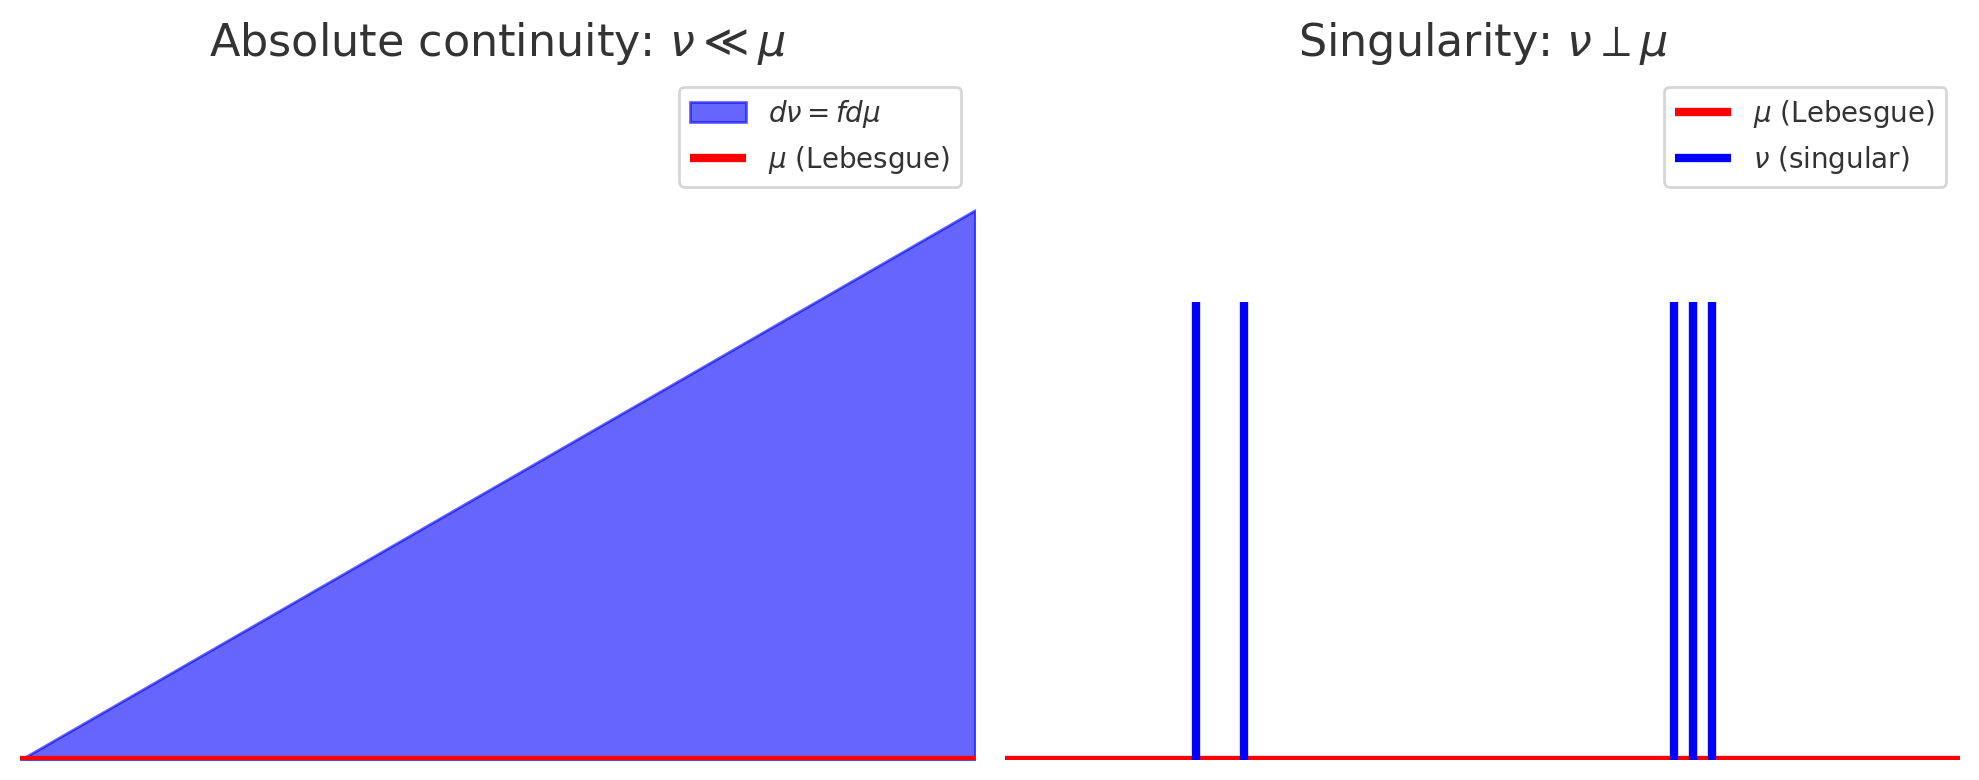
\includegraphics[width=0.65\linewidth]{fig/def4-10.png}
        \caption{Absolute continuous and Singular}
        \label{fig:def4.10}
    \end{figure}
\end{note}

\begin{note}{Thm 4.11}
Companion for Radon-Nikodym theorem.
\begin{enumerate}
    \item (Step 1). (1.a) $L^2(\mu)\subset L^1(\mu)$. If $f\in L^2(\mu)$ and $\mu$ is a finite measure ($\mu(E)<\infty$), then set $g\equiv 1$, by Cauchy-Schwarz inequality
    \[
    \int|f| \dif \mu \leq\left(\int|f|^{2} \dif \mu\right)^{1 / 2} \cdot(\mu(E))^{1 / 2}<\infty 
    \]
    So $f\in L^1(\mu)$, thus $L^2(\mu)\subset L^1(\mu)$.

    (1.b) Because we assume $v\le \mu$, if $\mu(A)=0$, then $v(A)\le \mu(A)=0$, thus $v\ll \mu$. Therefore \( f=\tilde{f},\ \mu \)-a.e. \( \Rightarrow f=\tilde{f},\ \nu \)-a.e.

    (1.c) Let $C=v(E)^{1/2}$, because $|\Phi(f)|\le C\|f\|_{L^2(\mu)}$, $\Phi(f)$ is a bounded linear map. Therefore it is continuous, see Proposition 1.3 in \href{https://ocw.mit.edu/courses/18-102-introduction-to-functional-analysis-spring-2021/3d4cc88026d44a01f936cd6a0aa995cb_MIT18_102s20_lec_FA.pdf}{MIT18.102}. So now we can apply Riesz.

    (1.d) Show $g\ge 0$. For every $\varepsilon>0$,
    \[
    \begin{aligned}
        \mu(\{x\in E:g(x)\le \varepsilon\})\ge v(\{x\in E:g(x)\le \varepsilon\})=\int_{\{x\in E:g(x)\le \varepsilon\}}g\dif \mu\ge \varepsilon\cdot \mu(\{x\in E:g(x)\le \varepsilon\})
    \end{aligned}
    \]
    So $\mu(\{x\in E:g(x)\le \varepsilon\})=0$, take a decreasing sequence of $\varepsilon\to 0$, then $\mu(\{x\in E:g(x)<0\})=0$. $g\ge 0\ \mu$ a.e..

    (1.e) The result of Step 1: Given a measure $\mu$, then there exists a $v\le \mu$ that is the measure of density $g$ with respect to $\mu$, i.e. $v=g\cdot \mu$ (see Cor 2.6),
    \[
    \int f\dif v=\int fg\dif \mu
    \]
    \item (Step 2). (2.a) We need $f$ to be a bounded measurable function for
    \[
    \int f \mathrm{~d} v=\int f h \mathrm{~d} \mu+\int f h \mathrm{~d} v\implies
    \int f (1-h)\mathrm{~d} v=\int f h \mathrm{~d} \mu
    \]
    To avoid $\infty-\infty$ in rearrangement, we need to show $\int f \mathrm{~d} v,\int f h \mathrm{~d} \mu$ and $\int f h \mathrm{~d} v$ are all finite. By $0\le h\le 1$, only need to show $\int f \mathrm{~d} v,\int f \mathrm{~d} \mu$ is finite. So if $f$ is bounded,
    \[
    \int |f| \mathrm{~d} v\le \sup |f|\cdot\int \mathrm{~d} v=\|f\|_{\infty}\cdot v(E)<\infty
    \]
    similar for $\mu$.

    (2.b) Then set $f_n:= f'\land n, f_n\uparrow f'$, so $f_n$ is bounded while $f'$ is any nonnegative measurable function.
    \[
    \int f' (1-h)\mathrm{~d} v=\lim_{n\to\infty}\int f_n(1-h)\mathrm{~d} v,\quad \int f' h\mathrm{~d} \mu=\lim_{n\to\infty}\int f_nh\mathrm{~d} \mu
    \]
    (2.c) $N=\{x\in E: h(x)=1\}$ is the founded $N$ such that $\mu(N)=0$, $v_s(N^c)=v(N^c\cap N)=0$, so $v_s \perp \mu$.

    (2.d) $\forall A\in\mathcal{A}, $ if $\mu(A)=0$, since $g=\mathbf{1}_{N^c}\frac{h}{1-h}$, then $v_a(A)=\int_A\dif v=\int_A g\dif\mu=\frac{h}{1-h}\mu(A\cap N^c)\le \frac{h}{1-h}\mu(A)=0$. So $v_a\ll \mu$.
    \item (Remark). Perfect counterexample. A counting measure $\mu$ on $([0,1],\mathcal{B}([0,1]))$ is not $\sigma$-finite because $[0,1]$ is uncountable. We need to find a sequence $\{A_n\}_n$ that $[0,1]=\bigcup_{n\ge 1}A_n, \mu(A_n)<\infty$ to make $\mu$ $\sigma$-finite. But a countable union of finite sets is at most countable. So $\mu$ cannot be $\sigma$-finite.
    \item (Conclusion). Given a measure $\mu$, consider a new measure $v$. Lebesgue decomposition says $v=v_a+v_s$. Radon-Nikodym theorem tells us there $\exists! g$, such that $v_a=g\cdot\mu$. In the proof, we also determined what exactly is $v_a,v_s$. So the process would be, first find a set $N$ where $\mu(N)=0$. Then 
    \[
    v_s=\mathbf{1}_N\cdot v,\quad v_a=\mathbf{1}_{N^c}\frac{\dif v}{\dif \mu}\cdot \mu
    \]
\end{enumerate}
\end{note}

\begin{note}{p.~80}
    Example (2). Consider measurable space $([0,1], \mathcal{F}_n)$, denote $f_n$ as the Radon-Nikodym derivative of $v$ with respect to $\lambda$. $\mathcal{F}_n=\sigma\left(I_i^{(n)};i\in\{1,2,\cdots,2^n\}\right)$ where
    \[
    I_i^{(n)}:=\left[ \frac{i-1}{2^n},\frac{i}{2^n} \right)
    \]
    Claim: $f_n(x)$ is constant on the atoms of $\mathcal{F}_n$. 
    \begin{proof}
        Recall Def 1.8, consider $((0,1],\mathcal{F}_n), (\mathbb{R},\mathcal{B}(\mathbb{R}))$, let $f_n:(0,1]\to \mathbb{R}$, $f_n$ is measurable, so
        \[
        \forall A\in \mathcal{B}(\mathbb{R}), f^{-1}_n(A)\in \mathcal{F}_n
        \]
        If $\exists a,b\in I_i^{(n)}, f_n(a)\neq f_n(b)$, then $f^{-1}(B_{\epsilon}(a))\subset I^{(n)}_i$ and $f^{-1}(B_{\epsilon}(a))\notin \mathcal{F}_n$.
    \end{proof}
    For $x\in I_i^{(n)}$, $f_n(x)=c_i$. Since $v=f_n\cdot \lambda$ by Radon-Nikodym theorem, 
    \[
    v(I_i^{(n)})=\int_{I_i^{(n)}}f_n(x)\lambda(\dif x)=c_i\lambda(I_i^{(n)})\implies c_i=\frac{v(I_i^{(n)})}{2^{-n}}
    \]
    since the Lebesgue measure $\lambda(I_i^{(n)})=2^{-n}$. So we conclude that 
    \[
    f_n(x)=\sum_{i=1}^{2^n}\mathbf{1}_{I_i^{(n)}}\frac{v(I_i^{(n)})}{2^{-n}}(x)
    \]
\end{note}
\setcounter{section}{4}
\section{Product Measures}

\begin{note}{Prop 5.1}
    (i) The goal is to show $\mathcal{C}=\mathcal{A}\otimes \mathcal{B}$. So $\mathcal{C}$ should contain all measurable rectangles like $\mathcal{A}\otimes \mathcal{B}$, and should be a $\sigma$-field.
    \begin{enumerate}
        \item $\forall A\in\mathcal{A},B\in\mathcal{B}$, let $C=A\times B\in\mathcal{C}$, then
        \[
        C_x=\{y\in F:(x,y)\in A\times B\}=\begin{cases}
            B & \text{if } x\in A\\
            \varnothing & \text{if } x\notin A
        \end{cases}
        \]
        \item $\mathcal{C}$ is a $\sigma$-field.
        \begin{enumerate}
            \item Let $C=E\times F,x\in E,C_x=F\in\mathcal{B}$, so $E\times F\in\mathcal{C}$
            \item If $C\in\mathcal{C}$, then $C_x\in\mathcal{B}$.
            \[
            (C^c)_x=\{y\in F:(x,y)\in (A\times B)^c\}=(C_x)^c\in\mathcal{B}
            \]
            since $\mathcal{B}$ is a $\sigma$-field and is closed under complements.
            \item If $C_n\in\mathcal{C}$, then $(C_n)_x\in\mathcal{B}$.
            \[
            \left(
            \bigcup_{n\ge 1}C_n
            \right)_x
            =\{y\in F:(x,y)\in\bigcup_{n\ge 1}C_n\}
            =\bigcup_{n\ge 1}\{y\in F:(x,y)\in C_n\}
            =\bigcup_{n\ge 1}(C_n)_x\in\mathcal{B}
            \]
            since $\mathcal{B}$ is a $\sigma$-field.
        \end{enumerate}
    \end{enumerate}
    (ii) The text already derived $f_x^{-1}(D)=(f^{-1}(D))_x$. Because $D\in\mathcal{G}$ and $f$ is measurable, $f^{-1}(D)\in \mathcal{A}\otimes\mathcal{B}$ by Def 1.8. By (i), $(f^{-1}(D))_x\in\mathcal{B}$, so $f_x^{-1}(D)\in\mathcal{B}$, which means $f_x$ is $\mathcal{B}$-measurable by Def 1.8. (ii) is the main result of this proposition, it tells us if $f:E\times F\to G$, then $f_x(y), f^y(x)$ are measurable on the corresponding $\sigma$-field of $y$ and $x$.
\end{note}

\begin{note}{Thm 5.2}
    A trick to show uniqueness is using $\sigma$-finite together with Cor 1.19. Another trick to show $x \mapsto v\left(C_{x}\right)$ is $\mathcal{A}$-measurable for all sets is constructing a class
    \[
    \mathcal{G} = \{ C \in \mathcal{A} \otimes \mathcal{B} : x \mapsto \nu(C_x) \text{ is } \mathcal{A}\text{-measurable} \}
    \]
    and show $\mathcal{G}$ equals the original $\sigma$-field $\mathcal{A}\otimes \mathcal{B}$. The structure is always: first suppose finite measures, then extend to $\sigma$-finite by restricting the measures on partitions of underlying set $E$.

    In this proof, we used Cor 1.19 for uniqueness. As for existence, assume $v$ is finite, define
    \[
    m(C):=\int_E v(C_x)\mu(\dif x).
    \]
    Consider the measurable spaces $(E,\mathcal{A},\mu)$ and $(F,\mathcal{B},v)$. Verify $v(C_x)$ is valid, that is $C_x\in \mathcal{B}$ (Prop 5.1). Then verify $x\mapsto\nu\left(C_{x}\right)$ is $\mathcal{A}$-measurable, so we can legally take integral (Thm 1.18). Now release $v$ from finite to $\sigma$-finite. Then check $m(C)$ is actually a measure (Def 1.6). Because 
    \[
    v(C_x)=\begin{cases}
        v(B) & \text{if }x\in A\\
        0 & \text{if }x\notin A
    \end{cases},\implies v(C_x)=\mathbf{1}_A(x) v(B)
    \]
    the property in (i) holds,
    \[
    m(C)=v(B)\int_E \mathbf{1}_A(x) \mu(\dif x)=v(B)\mu(A)
    \]
\end{note}

\begin{note}{Thm 5.3}
    We had a hard time proving Thm 5.2, which says
    \[
    \mu\otimes v(C)=\int_E v(C_x)\mu(\dif x)=\int_F \mu(C^y)v(\dif y).
    \]
    This is a special case of Thm 5.3 with $f=\mathbf{1}_{C}$, 
    \[
    \int_{E \times F} f \mathrm{~d} \mu \otimes v=\int_{E}\left(\int_{F} f(x, y) v(\mathrm{d} y)\right) \mu(\mathrm{d} x)=\int_{F}\left(\int_{E} f(x, y) \mu(\mathrm{d} x)\right) v(\mathrm{d} y)
    \]
    The extension from Thm 5.2 to 5.3 follows the route: indicator function $\to$ simple function $\to$ approximation (Prop 2.5(i)). Thm 5.3 applies only to nonnegative $f$, Thm 5.4 removed this condition. 
\end{note}

\begin{note}{p.~95}
    Write $\varphi(s,t)=\mathbf{1}_{\{s\le t\}}f(t)g(s)$, which is on space $([a,b],\mathcal{B}([a,b]),\lambda)\times ([a,b],\mathcal{B}([a,b]),\lambda)$. 
    
    Consider $h(s,t):=|f(t)g(s)|$ is nonnegative and measurable, apply Thm 5.3, 
    \[
    \begin{aligned}
        \int_{[a,b]^2}h(s,t)\dif (\lambda\otimes\lambda)
    &=\int_{a}^{b}\left(\int_{a}^{b}|f(t)||g(s)| \lambda(\dif s)\right) \lambda(\dif t)\\
     &=\int_{a}^{b}|f(t)|\left(\int_{a}^{b}|g(s)| \lambda(\dif s)\right) \lambda(\dif t)
      =\left(\int_{a}^{b}|g(s)| \dif s\right)\left(\int_{a}^{b}|f(t)| \dif t\right)
    \end{aligned}
    \]
    Notation $\lambda(\dif x)\iff \dif x$. Since $f,g$ are integrable, $\varphi(s,t)\in\mathcal{L}^1(\lambda\otimes\lambda)$. So
    \[
    \int_{a}^{b}\left(\int_{a}^{b} \varphi(s,t) \mathrm{d} s\right) \mathrm{d} t=\int_{a}^{b}\left(\int_{a}^{b} \varphi(s,t) \mathrm{d} t\right) \mathrm{d} s
    \]
\end{note}

\begin{note}{p.~100}
    Derive $I_n=n/(n+1)\cdot I_{n-2}$. By symmetry, $I_n=2\int_0^1 (1-x^2)^{n/2}\dif x$. Let $x=\sin\theta,\dif x=\cos\theta\dif\theta$, $x\in [0,1]\implies \theta\in[0,\pi/2]$.
    \[
    I_n = 2 \int_0^1 (1 - x^2)^{n/2} \dif x = 2 \int_0^{\pi/2} \cos^n \theta \cdot \cos \theta \, \dif\theta = 2 \int_0^{\pi/2} \cos^{n+1} \theta \, \dif\theta
    \]
    Integrate by part, let $u=\cos^n\theta,\dif v=\cos\theta\dif \theta$. This result in
    \[
    \int_0^{\pi/2} \cos^{n+1} \theta \, \dif\theta=n\int_0^{\pi/2} (1-\cos^2\theta)\cos^{n - 1} \theta \, \dif\theta\implies I_n=\frac{n}{n+1}I_{n-2}
    \]
\end{note}

\setcounter{section}{6}
\section{Change of Variables}

\begin{note}{Prop 7.1}
    (1) Given $A\in\mathcal{B}(\mathbb{R}^d)$, it is not guaranteed that $f(A)\in\mathcal{B}(\mathbb{R}^d)$, even though $f$ is continuous. It will always be Lebesgue measurable, but not necessarily Borel measurable. 

    Claim: All continuous functions are measurable.
    \begin{proof}
        Consider $(\mathbb{R}^d,\mathcal{B}(\mathbb{R}^d))$. $f:\mathbb{R}^d\to \mathbb{R}^d$ is continuous $\iff$ $\forall$ open set $U\subset \mathbb{R}^d$, $f^{-1}(U)$ is open in $\mathbb{R}^d$ (see Lemma 30 in \href{https://ocw.mit.edu/courses/18-s190-introduction-to-metric-spaces-january-iap-2023/mit18_s190iap23_lec2.pdf}{MIT18.S190 Lec2}). So if $f$ is continuous, then $\forall U\in \mathcal{B}(\mathbb{R}^d), f^{-1}(U)\in \mathcal{B}(\mathbb{R}^d)$. This is exactly the definition of $f$ being Boral measurable, Def 1.8.
    \end{proof}
    Since $M$ is invertible, $g:=f^{-1}$ is also continuous. Then $g^{-1}(A)$ is continuous, thus measurable. So $f(A)=(f^{-1})^{-1}(A)$ is measurable.

    (2) For special cases $P$ is orthonormal matrix and $S$ is symmetric positive definite, we have $1=|\det(P)|,c=|\det(S)|$. 
    \begin{lemma}[Polar Decomposition]
        Any invertible matrix $M$ can be decomposed as $M=PS$ where $P$ is an orthonormal matrix and $S$ is symmetric positive definite (spd).
    \end{lemma}
    \begin{proof}
        The intuition is rotate ($P$) and stretch out ($S$). If $M$ is invertible, then $M^TM$ is spd for sure. Let $S^2=M^TM$. Set $P=MS^{-1}$, now show that $P$ is orthonormal,
        \[
        P^TP=(MS^{-1})^TMS^{-1}=(S^{-1})^TM^TMS^{-1}=S^{-1}S^2S^{-1}=I
        \]
        So $M=PS$.
    \end{proof}
    Since $M$ is invertible, apply polar decomposition, $M=PS$ and $|\det(M)|=|\det(P)|\cdot|\det(S)|=c$.
\end{note}

\begin{note}{Thm 7.2}
    Let $f=\mathbf{1}_A$, then $f(\varphi(u))=\mathbf{1}_A(\varphi(u))=1$ only if $\varphi(u)\in A,u\in \varphi^{-1}(A)$, otherwise $f(\varphi(u))=0$. So $\int_U f(\varphi(u))|J_{\varphi}(u)|\dif u=\int_{\varphi^{-1}(A)}|J_{\varphi}(u)|\dif u$. Note that $A\subset D, B:=\varphi^{-1}(A)\subset U, \varphi(B)=A$. Replace $A$ by $\varphi(B)$, 
    \[
    \lambda_d(\varphi(B))=\int_{\varphi^{-1}(\varphi(B))}|J_{\varphi}(u)|\dif u=\int_B|J_{\varphi}(u)|\dif u
    \]
    The remaining proof is way too complicated, so skip it. Being able to use polar coordinates technique would be enough.
\end{note}

\begin{note}{p.~128}
    Recall equation (5.6),
    \[
    \gamma_{2k}=\frac{\pi^k}{k!},\quad \gamma_{2k+1}=\frac{\pi^k}{(k+\frac{1}{2})(k-\frac{1}{2})\cdots \frac{3}{2}\frac{1}{2}}
    \]
    and gamma function
    \[
    \Gamma(n)=(n-1)!,\quad \Gamma(\frac{1}{2}+n)=(n-\frac{1}{2})(n-\frac{3}{2})\cdots \frac{3}{2}\frac{1}{2}\sqrt{\pi}
    \]
    Consider $d=2k,k\in\mathbb{N}$ and $d=2k+1,k\in\mathbb{N}$ respectively,
    If $d=2k,k\in\mathbb{N}$, then 
    \[
    \gamma_{2k}=\frac{\pi^k}{\Gamma(k+1)}=\frac{\pi^{d/2}}{\Gamma(d/2+1)},\quad \gamma_{2k+1}=\frac{\pi^k\cdot\sqrt{\pi}}{\Gamma(\frac{1}{2}+k+1)}=\frac{\pi^{d/2}}{\Gamma(d/2+1)}
    \]
    It generates a unified form of volume for high-dimensional balls.
\end{note}
\part{Probability Theory}
\setcounter{section}{7}
\section{Foundations of Probability Theory}

\begin{note}{Def 8.2}
$\omega$ is hidden in formulas of probability theory.
\[
\mathbb{P}(X^{-1}(B))=\mathbb{P}(\{\omega\in\Omega:\omega\in X^{-1}(B)\})=\mathbb{P}(\{\omega\in\Omega:X(\omega)\in B\})=:\mathbb{P}(X\in B)
\]
\end{note}

\begin{note}{Prop 8.4}
    Review Fubini theorem, the only condition is $f\in\mathcal{L}^1(\mu\otimes v)$ and $\mu,v$ are $\sigma$-finite. In this case, $X$ is defined on $(\Omega,\mathcal{A},\mathbb{P})$.
    \[
    \{X\ge x\}=X^{-1}([x,+\infty))
    \]
    $X$ is a measurable function, $[x,+\infty)\subset \mathbb{R}$ is a Borel set, therefore $\{x\le X\}\in\mathcal{A}$ is a measurable subset in $\Omega$. $\mathbf{1}_{\{x\le X\}}:\Omega\to\{0,1\}$, check $\forall B\in\mathcal{P}(\{0,1\}),$  so $B\in\mathcal{B}(\mathbb{R})$,
    \[
    \mathbf{1}_{\{x\le X\}}^{-1}(B)=\{\omega\in\Omega: \mathbf{1}_{\{x\le X\}}(\omega)\in B\}\in\mathcal{A}
    \]
    so $\mathbf{1}_{\{x\le X\}}$ is a Lebesgue measurable function. $\mathbf{1}_{\{x\le X\}}\in \mathcal{L}^1(\mathbb{P}\otimes \lambda)$, Fubini theorem is applicable.
\end{note}

\begin{note}{Prop 8.5}
    Recall Prop 2.9,
    \[
    \int_E h(\varphi(x))\mu(\dif x)=\int_F h(y)v(\dif y)
    \]
    here $\mu=\mathbb{P},v=\mathbb{P}_X,\varphi=X$,
    \[
    \mathbb{E}[f(X)]=\int_{\Omega}f(X(\omega))\mathbb{P}(\dif\omega)=\int_E f(x)\mathbb{P}_X(\dif x)
    \]
\end{note}

\begin{note}{p.~142}
    In the discussion after Prop 8.5, the text
    \begin{quote}
        Since the indicator function of an open rectangle is the increasing limit of a sequence of continuous functions with compact support, the probability measure \( \mu \) is also determined by the values of \( \int \varphi(x) \mu(\mathrm{d} x) \) when \( \varphi \) varies in the space \( C_{c}\left(\mathbb{R}^{d}\right) \) of all continuous functions with compact support from \( \mathbb{R}^{d} \) into \( \mathbb{R} \). 
    \end{quote}
    means any indicator function of a rectangle $\mathbf{1}_R$ can be approximated from below by a sequence $\varphi_n\in C_c(\mathbb{R}^d)$. See a construction of Lemma 2.2 in \href{https://ocw.mit.edu/courses/18-102-introduction-to-functional-analysis-spring-2021/3d4cc88026d44a01f936cd6a0aa995cb_MIT18_102s20_lec_FA.pdf}{MIT18.102}. So
    \[
    \mathbf{1}_R(x) = \lim_{n \to \infty} \varphi_n(x) \quad \text{with each } \varphi_n \in C_c(\mathbb{R}^d), \; \varphi_n \leq \mathbf{1}_R
    \]
    By the \emph{monotone convergence theorem},
    $$
    \mu(R) = \int \mathbf{1}_R(x) \, \mu(dx) = \lim_{n \to \infty} \int \varphi_n(x) \, \mu(dx)
    $$
\end{note}

\begin{note}{Prop 8.9}
    $\mathbf{1}_{A_i}=\mathbf{1}_{B_i}\circ X$. 
    \[
1_{A_i}(\omega) = \begin{cases}
1 & \text{if } \omega \in A_i, \\
0 & \text{otherwise},
\end{cases}
= \begin{cases}
1 & \text{if } X(\omega) \in B_i, \\
0 & \text{otherwise},
\end{cases}
= 1_{B_i}(X(\omega)) = (1_{B_i} \circ X)(\omega).
\]
\end{note}

\begin{note}{p.~153}
    Show Markov inequality. Let $A_a=\{\omega\in\Omega: X(\omega)\ge a\}, X\ge a\mathbf{1}_{A_a}.$ 
    \[
    \int X\dif \mathbb{P}\ge a\int\mathbf{1}_{A_a}\dif \mathbb{P}=a\mathbb{P}(A_a),\implies \mathbb{P}(A_a)\le\frac{1}{a}\int\mathbf{1}_{A_a}\dif \mathbb{P}=\frac{1}{a}\mathbb{E}[X]
    \]
\end{note}

\begin{note}{Prop 8.13}
    Given $\alpha_0=\mathbb{E}[X]$ in equation (8.5), then 
    \[
    Z=\mathbb{E}[X]+\sum_{j=1}^n \alpha_j (Y_j-\mathbb{E}[Y_j])
    \]
    To let equation (8.6) holds, plug in $Z$,
    \[
    \mathbb{E}[(X-\mathbb{E}[X])(Y_k-\mathbb{E}[Y_k])]-\sum_{j=1}^n \alpha_j \mathbb{E}[(Y_j-\mathbb{E}[Y_j])(Y_k-\mathbb{E}[Y_k])]=0
    \]
    This is exactly $\text{cov}(X,Y_k)=\sum_{j=1}^n \alpha_j\text{cov}(Y_j,Y_k)$.
\end{note}

\begin{note}{Def 8.14}
    A probability measure is absolutely continuous with respect to Lebesgue measure if and only if it has a density function $\varphi(x)$. Then applies Radon-Nikodym theorem, $\mathbb{P}_X(\dif x)=\varphi(x)\lambda(\dif x)$. Recall \emph{Fourier Transform} in p.~32,
    \[
    \hat{\varphi}(\xi)=\int e^{i\xi x}\varphi(x)\lambda(\dif x)=\int e^{i\xi x}\mathbb{P}_X(\dif x)=:\Phi(\xi)
    \]
\end{note}

\begin{note}{Lem 8.15}
    (1) Parity argument: $e^{i\xi X}=\cos(\xi X)+i\sin(\xi X)$.

    (2) To use Thm 2.13, let $h(u,x)=e^{-x^2/2}\cos(ux)$, find a function $g(x)$ such that 
    \[
    |h(u,x)-h(\xi,x)|\le g(x)\cdot |u-\xi|
    \]
    By mean value theorem, $\exists c\in(u,\xi)$ (or $(\xi,u)$), such that $|\cos(ux)-\cos(\xi x)|=|-x\sin(cx)||u-\xi|.$
    \[
    |e^{-x^2/2}(\cos(ux)-\cos(\xi x))|\le e^{-x^2/2}|\cos(ux)-\cos(\xi x)|\le e^{-x^2/2}|x|\cdot|u-\xi|=g(x)\cdot|u-\xi|
    \]
    where $g(x)=|x|\cdot e^{-x^2/2}\in\mathcal{L}^1_+$. So condition (ii) satisfies.

    (3) If $Z\sim \mathcal{N}(0,1)$, then $\Phi_Z(\xi)=\exp(-\xi^2/2)$. For $X=m+\sigma Z\sim \mathcal{N}(m,\sigma^2)$,
    \[
    \Phi_X(\xi)=\mathbb{E}[\exp(i\xi X)]=\mathbb{E}[\exp(i\xi (m+\sigma Z))]=e^{i\xi m}\cdot \Phi_Z(\sigma\xi)=e^{i\xi m}\cdot e^{-\sigma^2\xi^2/2}
    \]
\end{note}

\begin{note}{Thm 8.16}
    (i) To establish (1), use Lem 8.15 to find that $X\sim\mathcal{N}(0,1/\sigma)$, and use Def 8.14 to write
    \[
    \exp(-\frac{x^2}{2\sigma^2})= \Phi_X(x)= \int_{\mathbb{R}}e^{ix\cdot \xi}g_{1/\sigma}(\xi)\dif \xi
    \]
\end{note}
\setcounter{section}{8}
\section{Independence}

\begin{note}{p.~170}
    Given $X_j$ is in $(E_j,\mathcal{E}_j)$. The following expressions are equivalent:
    \begin{enumerate}
        \item $\mathbb{P}(A_j)$: $A_j$ is an element in $\sigma(X_j)$
        \item $\mathbb{P}(\{X_j\in F_j\})$: $F_j$ is an element in $\mathcal{E}_j$
    \end{enumerate}
    In (1), $\sigma(X_j)=\{X_j^{-1}(F):F\in\mathcal{E}_j\}$. An element in $\sigma(X_j)$ means for some $F_j\in\mathcal{E}_j$, $A_i=\{X_j^{-1}(F_j)\}=\{\omega\in\Omega:X_j(\omega)\in F_j\}$. This is exactly $\{X_j\in F_j\}$ in (2).
\end{note}

\begin{note}{Thm 9.4}
    In Thm 5.2(1), $\mu\otimes v(A\times B)=\mu(A)v(B)$, so 
    \[
    \mathbb{P}_{X_{1}} \otimes \cdots \otimes \mathbb{P}_{X_{n}}\left(F_{1} \times \cdots \times F_{n}\right)=\prod_{i=1}^{n} \mathbb{P}_{X_{i}}\left(F_{i}\right)
    \]
\end{note}

\begin{note}{Prop 9.7}
    Check that $\mathcal{M}_1$ is a monotone class.
    
    (i) Let $C_1=\Omega$, then $\Omega\in\mathcal{M}_1$.  (ii) If $B,B'\in\mathcal{M}_1$ and $B\subset B'$, 
    \[
    \mathbb{P}(B'\cap C_2\cap\cdots\cap C_n)=\mathbb{P}(B\cap C_2\cap\cdots\cap C_n)+\mathbb{P}((B'\setminus B)\cap C_2\cap\cdots\cap C_n)
    \]
    and 
    \[
    \mathbb{P}((B'\setminus B)\cap C_2\cap\cdots\cap C_n)=(\mathbb{P}(B')-\mathbb{P}(B))\cdot\mathbb{P}(C_2)\cdots\mathbb{P}(C_n)=\mathbb{P}(B'\setminus B)\mathbb{P}(C_2)\cdots\mathbb{P}(C_n)
    \]
    Thus $B'\setminus B\in\mathcal{M}_1$. (iii) If $\{B_j\}\in\mathcal{M}_1$, where $B_j\subset B_{j+1}$,
    \[
    \begin{aligned}
        \mathbb{P}\left((\bigcup_{j=1}^{\infty}B_j)\cap C_2\cap\cdots\cap C_n\right)
        &=\mathbb{P}\left(\bigcup_{j=1}^{\infty}(B_j\cap C_2\cap\cdots\cap C_n)\right)\\
        &=\lim_{j\to\infty}\uparrow \mathbb{P}\left(B_j\cap C_2\cap\cdots\cap C_n\right)\\
        &=\lim_{j\to\infty}\uparrow \mathbb{P}(B_j)\mathbb{P}(C_2)\cdots\mathbb{P}(C_n)\\
        &=\mathbb{P}\left(
        \bigcup_{j=1}^{\infty}B_j
        \right)\mathbb{P}(C_2)\cdots\mathbb{P}(C_n)
    \end{aligned}
    \]
    Thus $\bigcup_{j=1}^{\infty}B_j\in\mathcal{M}_1$.
\end{note}

\begin{note}{p.~175}
    For every $j\in\{1,\cdots,p\}$, construct
    \[
    \mathcal{C}_j=\{B_{n_{j-1}+1}\cap\cdots\cap B_{n_j}: B_i\in\mathcal{B}_i,i\in\{n_{j-1}+1,\cdots,n_j\}\}
    \]
    Show $\mathcal{C}_j$ is closed under finite intersections. Consider $\mathcal{C}_j^{(1)},\mathcal{C}_j^{(2)}$, then
    \[
    \mathcal{C}_j^{(1)}\cap\mathcal{C}_j^{(2)}=\left(
    \bigcap_{i=n_{j-1}+1}^{n_j}B_i^{(1)}
    \right)\cap\left(
    \bigcap_{i=n_{j-1}+1}^{n_j}B_i^{(2)}
    \right)=\bigcap_{i=n_{j-1}+1}^{n_j}(B_i^{(1)}\cap B_i^{(2)})
    \]
    and $B_i^{(1)}\cap B_i^{(2)}\in\mathcal{B}_i$ because $\mathcal{B}_i$ is closed under finite intersections. So $\mathcal{C}_j^{(1)}\cap\mathcal{C}_j^{(2)}\in\mathcal{C}_j$.
\end{note}

\begin{note}{Lem 9.11}
    Show that $\sum\mathbb{P}(A_k)=\infty$ implies $\prod_{k=n_0}^n (1-\mathbb{P}(A_k))=0$. For $0<x<1,\ln(1-x)<-x$. Let $x=\mathbb{P}(A_k)$, then $\ln(1-\mathbb{P}(A_k))<-\mathbb{P}(A_k)$.
    \[
    \ln\prod_{k=n_0}^n (1-\mathbb{P}(A_k))=\sum_{k=n_0}^n\ln(1-\mathbb{P}(A_k))\le -\sum_{k=n_0}^n\mathbb{P}(A_k)\to -\infty
    \]
    So $\prod_{k=n_0}^n(1-\mathbb{P}(A_k))\to 0$ as $n\to\infty$.
\end{note}

\begin{note}{p.~179}
Show $X_n(\omega)\in \{0,1\}.$ For all $t\in\mathbb{R}, 2\lfloor t\rfloor\le\lfloor 2t\rfloor\le 2\lfloor t\rfloor+1$. Let $t=2^{n-1}\omega$, then $\lfloor 2t\rfloor-2\lfloor t\rfloor\in\{0,1\}$. Since $\omega\in[0,1), \lfloor \omega\rfloor=0$.
$$
\begin{aligned}
\sum_{k=1}^n X_k(\omega)\,2^{\,n-k}
&=\sum_{k=1}^n\big(\lfloor 2^k\omega\rfloor-2\lfloor 2^{k-1}\omega\rfloor\big)2^{\,n-k}\\
&=\sum_{k=1}^n\lfloor 2^k\omega\rfloor\,2^{\,n-k}-\sum_{k=1}^n\lfloor 2^{k-1}\omega\rfloor\,2^{\,n-k+1}\\
&=\sum_{j=1}^n\lfloor 2^j\omega\rfloor\,2^{\,n-j}-\sum_{j=0}^{n-1}\lfloor 2^{j}\omega\rfloor\,2^{\,n-j}\\
&=\lfloor 2^n\omega\rfloor-\lfloor 2^0\omega\rfloor\,2^{\,n}
=\lfloor 2^n\omega\rfloor
\end{aligned}
$$
So $0\le 2^n\omega-\sum_{k=1}^n X_k(\omega)\,2^{\,n-k}=2^n\omega-\lfloor 2^n\omega\rfloor<1$. Divide both sides by $2^n$ and get the desired result.
\end{note}

\begin{note}{p.~182}
    $\mu *v$ is the pushforward measure of $\mu\otimes v$ under $f(x,y)=x+y$, i.e. $\forall B\in \mathbb{R}^d, \mu *v(B)=\mu\otimes v (f^{-1}(B))$. By Prop 2.9,
    \[
    \int_{\mathbb{R}^d} \varphi(z)\mu*z(\dif z)
    =\int_{\mathbb{R}^d\times \mathbb{R}^d}\varphi(f(x,y))\dif \mu\otimes v
    =\int_{\mathbb{R}^d}\int_{\mathbb{R}^d}\varphi(x+y)\mu(\dif x)v(\dif y)
    \]
\end{note}

\begin{note}{Prop 9.12}
    Proof of (i). Trick: When finding the \emph{law} of some random variable $X$, check $\mathbb{E}[\varphi(X)]$ for every \emph{nonnegative measurable} function $\varphi$ (in order to use Fubini theorem). Same trick is used at the \emph{Example} on p.~174.
\end{note}

\begin{note}{Thm 9.13}
    Derive the last equation. Denote $X=X_1+\cdots +X_n, \text{var}(X)=\mathbb{E}[X^2]-(\mathbb{E}[X])^2$. $\mathbb{E}[X^2]=\text{var}(X)+(\mathbb{E}[X])^2=\text{var}(X)+n^2(\mathbb{E}[X_1])^2$. So
    \[
    \begin{aligned}
    \mathbb{E}\left[
    \left(
    \frac{1}{n}X-\mathbb{E}[X_1]
    \right)^2
    \right]
    &=\frac{1}{n^2}\mathbb{E}[X^2]-\frac{2}{n}\mathbb{E}[X]\cdot\mathbb{E}[X_1]+(\mathbb{E}[X_1])^2\\
    &=\frac{1}{n^2}\text{var}(X)+(\mathbb{E}[X_1])^2-2(\mathbb{E}[X_1])^2+(\mathbb{E}[X_1])^2=\frac{1}{n^2}\text{var}(X) 
    \end{aligned}
    \]
\end{note}



\end{document}
